\documentclass[12pt, twoside]{article}
\usepackage[letterpaper, margin=1in, headsep=0.5in]{geometry}
\usepackage[english]{babel}
\usepackage[utf8]{inputenc}
\usepackage{amsmath}
\usepackage{amsfonts}
\usepackage{amssymb}
\usepackage{tikz}
\usetikzlibrary{quotes, angles}
\usepackage{graphicx}
\usepackage{enumitem}
\usepackage{multicol}

\newif\ifmeta
\metatrue %print standards and topics tags

\title{Regents Geometry}
\author{Chris Huson}
\date{September 2020}

\usepackage{fancyhdr}
\pagestyle{fancy}
\fancyhf{}
\renewcommand{\headrulewidth}{0pt} % disable the underline of the header
\raggedbottom


\fancyhead[LE]{\thepage}
\fancyhead[RO]{\thepage \\ Name: \hspace{4cm} \,\\}
\fancyhead[LO]{BECA / Dr. Huson / Geometry 07-Similarity\\* pset ID: 113}

\begin{document}

\subsubsection*{7-6DN-Symmetry}
\begin{enumerate}
\item A translation maps triangle $PQR$ onto triangle $STU$. \vspace{0.5cm}
  \begin{multicols}{2}
    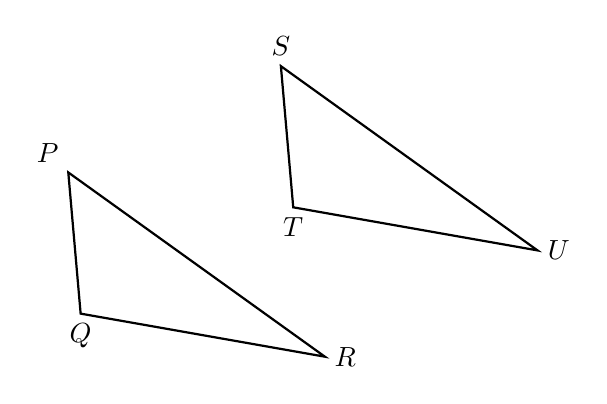
\begin{tikzpicture}[scale=0.9]
      \coordinate [label=above left:$P$](A) at (95:2);
      \coordinate [label=below:$Q$](B) at (0, 0);
      \coordinate [label=right:$R$](C) at (-10:3.5);
      \draw [thick] (A)--(B)--(C)--cycle;

      \draw [thick, xshift=3cm, yshift=1.5cm] (95:2) node[above]{$S$}--
      (0,0) node[below]{$T$}--
      (-10:3.5) node[right]{$U$}--cycle;
    \end{tikzpicture}\\
    Write each corresponding object.
    \begin{enumerate}
      \item $Q \rightarrow$ \rule{2cm}{0.15mm}
      \item $\angle QRP \cong$ \rule{2cm}{0.15mm}
      \item \rule{2cm}{0.15mm} $\cong \overline {ST}$
      \item Justify $\triangle PQR \cong \triangle STU$. Use the words ``rigid motion".
    \end{enumerate}
    \end{multicols}  \vspace{2cm}

\item Given $\triangle JKL \sim \triangle MNO$. $m\angle K = 40^\circ$ and $m\angle M = 100^\circ$.\\
  Find the measure of $\angle L$. \vspace{3cm}

\item Triangle $ABC$ is dilated with a scale factor of $k$ centered at $A$, yielding $\triangle ADE$, as shown. Given $AB=8$, $BC=10$, $AC=12$, and $DE=15$. \\[0.25cm] Find $AD$, $CE$, and $k$ (the scale factor). \vspace{0.5cm}
  \begin{center}
      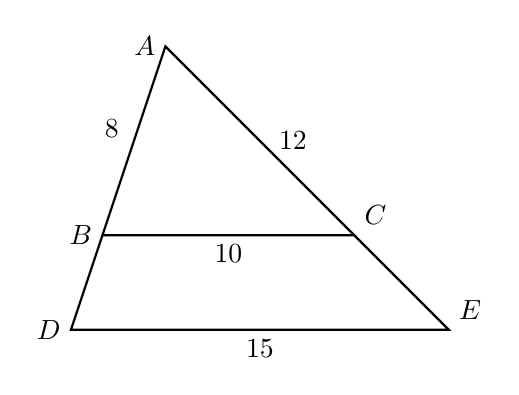
\begin{tikzpicture}[scale=0.4]
        \draw [thick]
        (0,0)node[left]{$B$}--
        (8,0)node[above right]{$C$}--
        (2,6)node[left]{$A$}--cycle;
        \draw [thick]
        (0,0)--
        (-1,-3)node[left]{$D$}--
        (11,-3)node[above right]{$E$}--(8,0);
        \node at (4,0)[below]{$10$};
        \node at (5.3, 3)[right]{$12$};
        \node at (0.3, 2.8)[above]{$8$};
        \node at (5,-3)[below]{$15$};
      \end{tikzpicture}
    \end{center}
    
\newpage

\item What transformation maps $\triangle ABC$ onto $\triangle DEC$, shown below? Fully specify the transformation.
    \begin{flushright}
      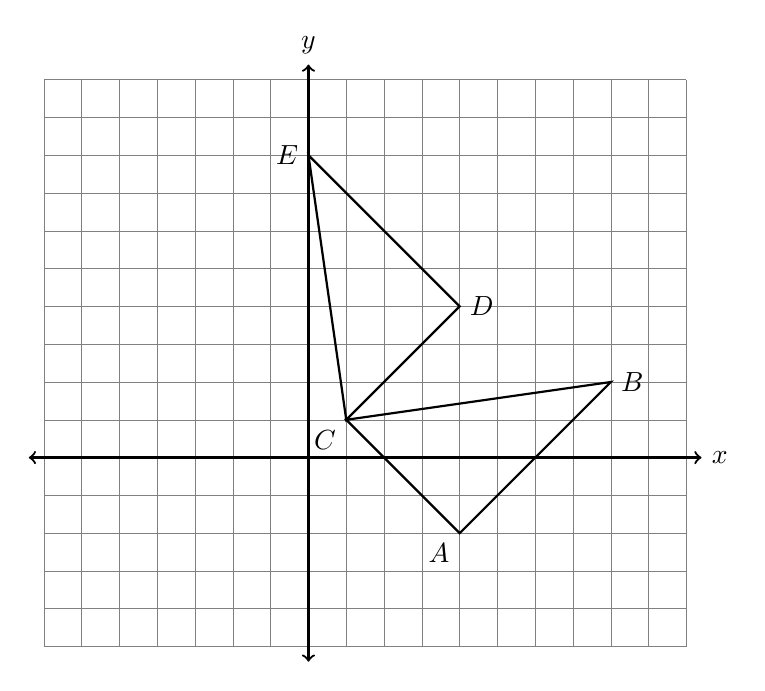
\begin{tikzpicture}[scale=.48]
        \draw [help lines] (-7,-5) grid (10,10);
        \draw [thick, <->] (-7.4,0) -- (10.4,0) node [right] {$x$};
        \draw [thick, <->] (0,-5.4)--(0,10.4) node [above] {$y$};
        \draw [thick]
        (4,-2) node[below left] {$A$}--
        (8,2) node[right] {$B$}--
        (1,1) node[below left] {$C$}--cycle;
        \draw [thick]
        (4,4) node[right] {$D$}--
        (0,8) node[left] {$E$}--
        (1,1) --cycle;
      \end{tikzpicture}
    \end{flushright}

\item What is the smallest non-zero angle of rotation about its center that would map the equilateral triangle onto itself?
  \begin{center}
      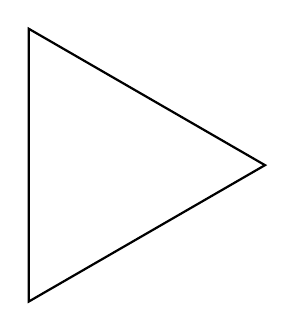
\begin{tikzpicture}%[scale=.48]
        \draw [thick]
        (0:2)--
        (120:2)--
        (240:2)--cycle;
      \end{tikzpicture}
    \end{center}
  
\item Given right $\triangle ABC$ with $\overline{AC} \perp \overline{BC}$, $BC=11.2$, $m\angle B=63^\circ$. Let $x=AC$. Find $x$.
  \begin{flushright}
    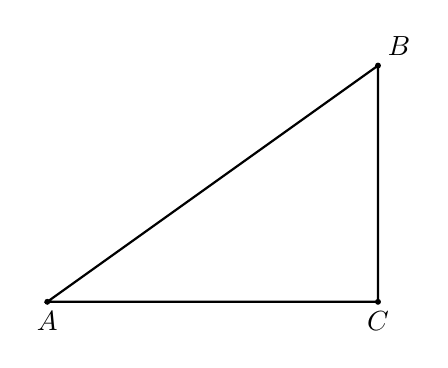
\begin{tikzpicture}[scale=0.6]
      \draw [thick](-1,0)--(6,0)--(6,5)--cycle;
      \draw [fill] (-1,0) circle [radius=0.05] node[below]{$A$};
      \draw [fill] (6,0) circle [radius=0.05] node[below]{$C$};
      \draw [fill] (6,5) circle [radius=0.05] node[above right]{$B$};
    \end{tikzpicture}
  \end{flushright}

\end{enumerate}
\end{document}